\section{Data Retrieval}
Our data sets (\textbf{Medical Cost Personal Datasets}) were obtained from the \texttt{Kaggle} website\cite{kaggle:2022a}.

The data set has six independent variables:
\begin{enumerate}
\item \texttt{age} 
\item \texttt{sex} 
\item \texttt{bmi} 
\item \texttt{children} 
\item \texttt{smoker}
\item \texttt{region}	
\end{enumerate}
and one dependent variable: \texttt{charge}.

In Fig.\,\ref{fig:chargesfuncofbmi} the charges (\$) as function of bmi are displayed.
\begin{figure}[h]
   \centering
	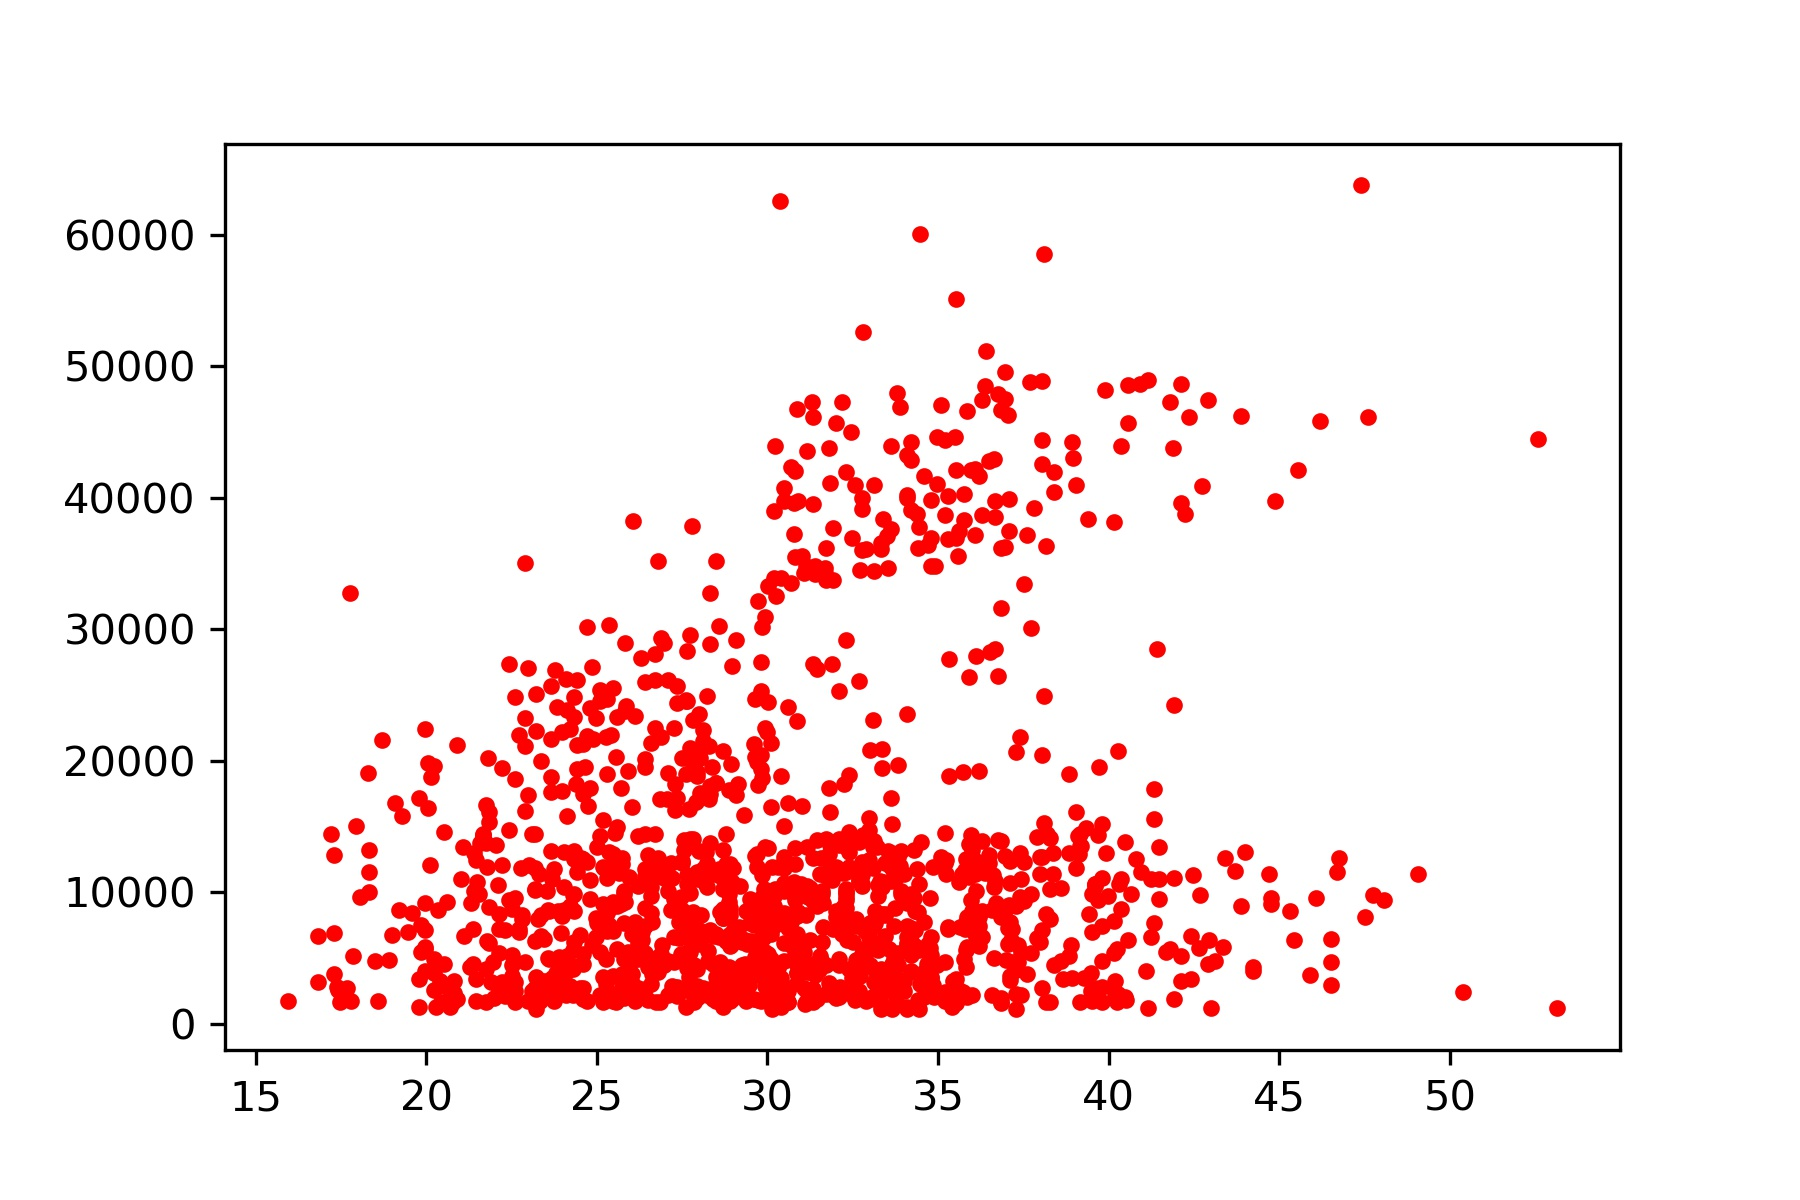
\includegraphics{../img/imgpy1.jpeg}
	\caption{Charges (\$) as function of bmi.}
  \label{fig:chargesfuncofbmi}
\end{figure}

In Fig.\,\ref{fig:countsofage} the age histogram is displayed.
\begin{figure}[h]
   \centering
        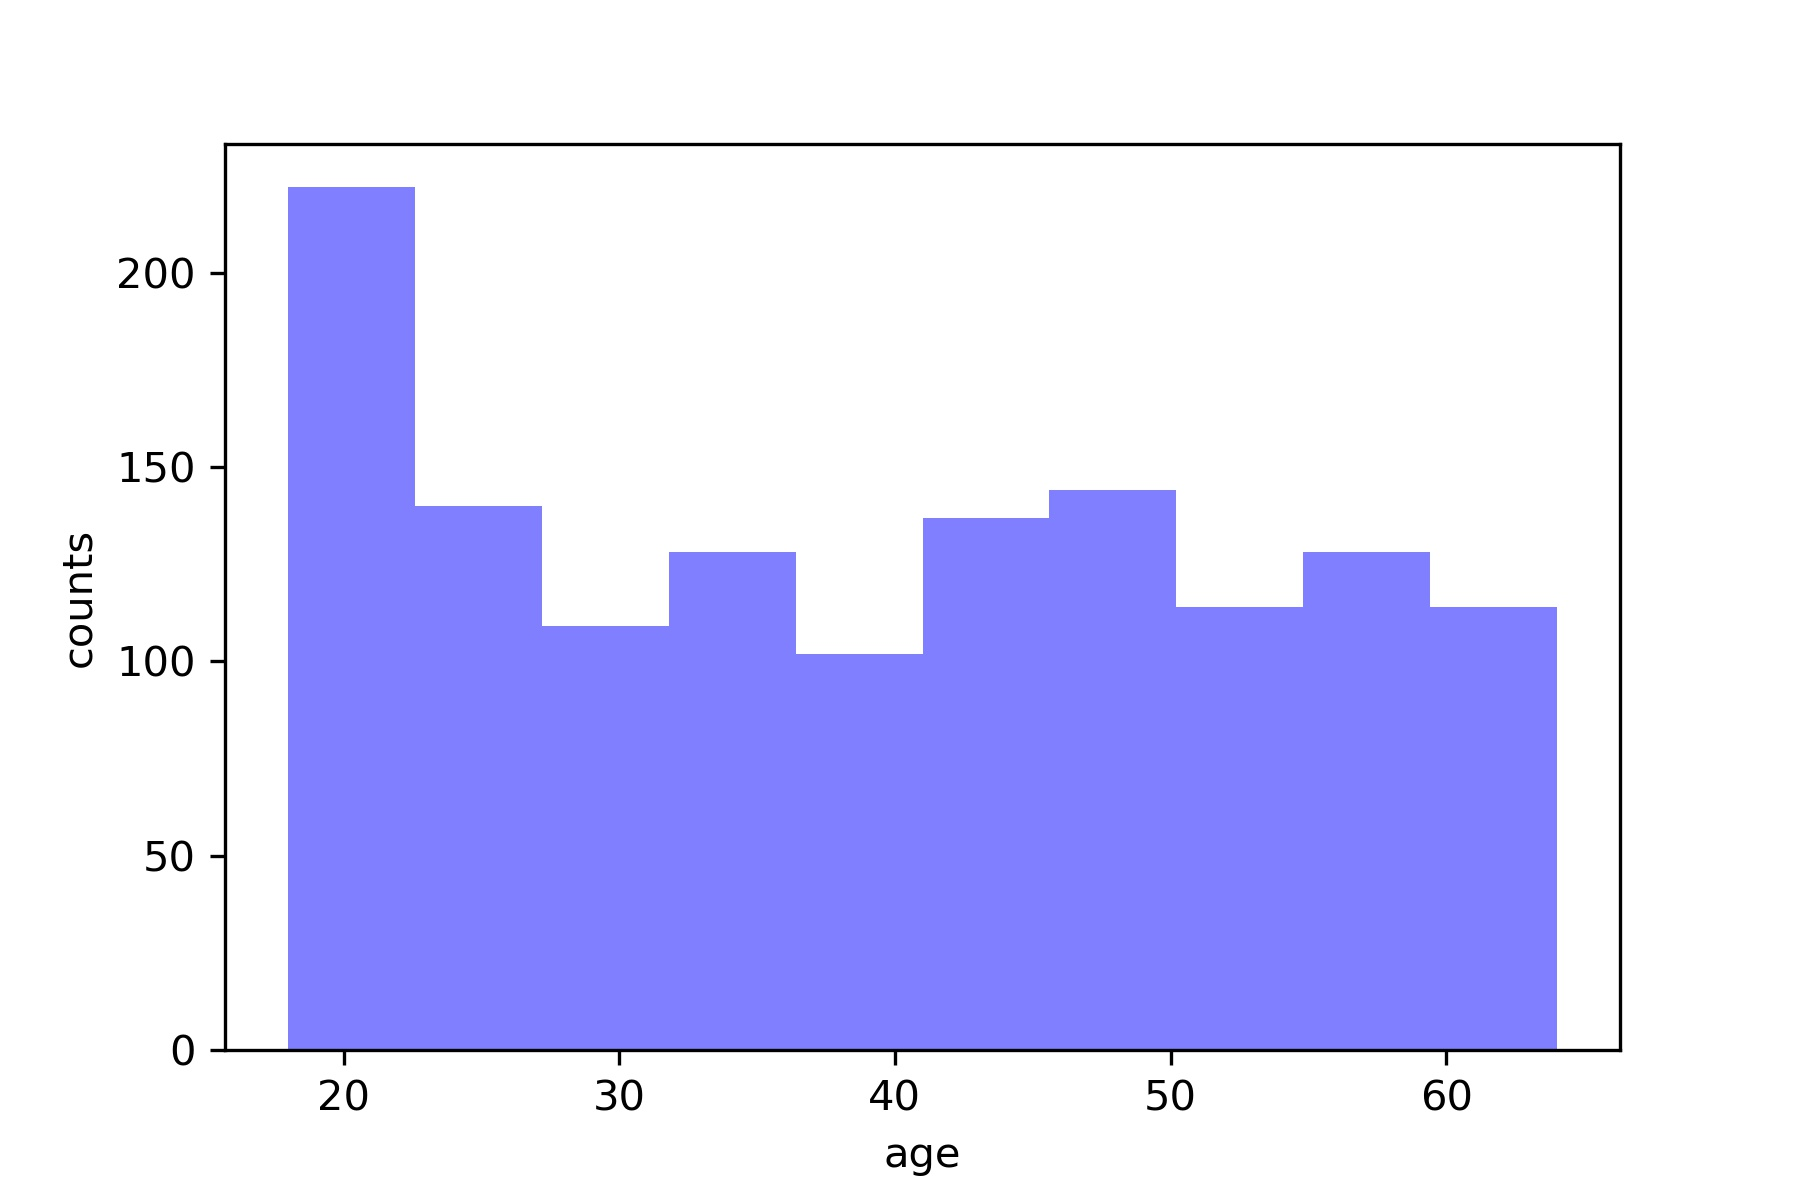
\includegraphics{../img/imgpy2.jpeg}
        \caption{Age histogram.}
  \label{fig:countsofage}
\end{figure}

